%\documentclass{article}
% Include all project wide packages here.
\usepackage{fullpage}
\usepackage{polyglossia}
\setmainlanguage{dutch}
\usepackage{csquotes}
\usepackage{graphicx}
\usepackage{epstopdf}
\usepackage{pdfpages}
\usepackage{caption}
\usepackage[list=true]{subcaption}
\usepackage{float}
%\usepackage{mathtools}
\usepackage{standalone}
\usepackage{import}
\usepackage{tocloft}
\usepackage{wrapfig}
\usepackage{authblk}
\usepackage{array}
\usepackage{booktabs}
\usepackage[toc,page,title,titletoc]{appendix}
\usepackage{xunicode}
\usepackage{amsmath}
\usepackage{fontspec}
\usepackage{unicode-math}
\usepackage[
    backend=bibtexu,
	texencoding=utf8,
bibencoding=utf8,
    style=ieee,
    sortlocale=nl_NL,
    language=auto
]{biblatex}
\usepackage{listings}
\newcommand{\includecode}[3][c]{\lstinputlisting[caption=#2, escapechar=, style=#1]{#3}}
\newcommand{\superscript}[1]{\ensuremath{^{\textrm{#1}}}}
\newcommand{\subscript}[1]{\ensuremath{_{\textrm{#1}}}}


\newcommand{\chapternumber}{\thechapter}
\renewcommand{\appendixname}{Bijlage}
\renewcommand{\appendixtocname}{Bijlagen}
\renewcommand{\appendixpagename}{Bijlagen}

\usepackage[hidelinks]{hyperref} %<--------ALTIJD ALS LAATSTE

\renewcommand{\familydefault}{\sfdefault}

\setmainfont[Ligatures=TeX]{Myriad Pro}
\setmathfont{Asana Math}
\setmonofont{Lucida Console}

\usepackage{titlesec, blindtext, color}
\definecolor{gray75}{gray}{0.75}
\newcommand{\hsp}{\hspace{20pt}}
\titleformat{\chapter}[hang]{\Huge\bfseries}{\chapternumber\hsp\textcolor{gray75}{|}\hsp}{0pt}{\Huge\bfseries}
\renewcommand{\familydefault}{\sfdefault}
\renewcommand{\arraystretch}{1.2}
\setlength\parindent{0pt}

%For code listings
\definecolor{black}{rgb}{0,0,0}
\definecolor{browntags}{rgb}{0.65,0.1,0.1}
\definecolor{bluestrings}{rgb}{0,0,1}
\definecolor{graycomments}{rgb}{0.4,0.4,0.4}
\definecolor{redkeywords}{rgb}{1,0,0}
\definecolor{bluekeywords}{rgb}{0.13,0.13,0.8}
\definecolor{greencomments}{rgb}{0,0.5,0}
\definecolor{redstrings}{rgb}{0.9,0,0}
\definecolor{purpleidentifiers}{rgb}{0.01,0,0.01}


\lstdefinestyle{csharp}{
language=[Sharp]C,
showspaces=false,
showtabs=false,
breaklines=true,
showstringspaces=false,
breakatwhitespace=true,
escapeinside={(*@}{@*)},
columns=fullflexible,
commentstyle=\color{greencomments},
keywordstyle=\color{bluekeywords}\bfseries,
stringstyle=\color{redstrings},
identifierstyle=\color{purpleidentifiers},
basicstyle=\ttfamily\small}

\lstdefinestyle{c}{
language=C,
showspaces=false,
showtabs=false,
breaklines=true,
showstringspaces=false,
breakatwhitespace=true,
escapeinside={(*@}{@*)},
columns=fullflexible,
commentstyle=\color{greencomments},
keywordstyle=\color{bluekeywords}\bfseries,
stringstyle=\color{bluestrings},
identifierstyle=\color{purpleidentifiers}
}

\lstdefinestyle{vhdl}{
language=VHDL,
showspaces=false,
showtabs=false,
breaklines=true,
showstringspaces=false,
breakatwhitespace=true,
escapeinside={(*@}{@*)},
columns=fullflexible,
commentstyle=\color{greencomments},
keywordstyle=\color{bluekeywords}\bfseries,
stringstyle=\color{redstrings},
identifierstyle=\color{purpleidentifiers}
}

\lstdefinestyle{xaml}{
language=XML,
showspaces=false,
showtabs=false,
breaklines=true,
showstringspaces=false,
breakatwhitespace=true,
escapeinside={(*@}{@*)},
columns=fullflexible,
commentstyle=\color{greencomments},
keywordstyle=\color{redkeywords},
stringstyle=\color{bluestrings},
tagstyle=\color{browntags},
morestring=[b]",
  morecomment=[s]{<?}{?>},
  morekeywords={xmlns,version,typex:AsyncRecords,x:Arguments,x:Boolean,x:Byte,x:Char,x:Class,x:ClassAttributes,x:ClassModifier,x:Code,x:ConnectionId,x:Decimal,x:Double,x:FactoryMethod,x:FieldModifier,x:Int16,x:Int32,x:Int64,x:Key,x:Members,x:Name,x:Object,x:Property,x:Shared,x:Single,x:String,x:Subclass,x:SynchronousMode,x:TimeSpan,x:TypeArguments,x:Uid,x:Uri,x:XData,Grid.Column,Grid.ColumnSpan,Click,ClipToBounds,Content,DropDownOpened,FontSize,Foreground,Header,Height,HorizontalAlignment,HorizontalContentAlignment,IsCancel,IsDefault,IsEnabled,IsSelected,Margin,MinHeight,MinWidth,Padding,SnapsToDevicePixels,Target,TextWrapping,Title,VerticalAlignment,VerticalContentAlignment,Width,WindowStartupLocation,Binding,Mode,OneWay,xmlns:x}
}

%defaults
\lstset{
basicstyle=\ttfamily\small,
extendedchars=false,
numbers=left,
numberstyle=\ttfamily\tiny,
stepnumber=1,
tabsize=4,
numbersep=5pt
}



\begin{document}
\subsection{Implementatie}
\begin{itemize}
\item Nadat de VHDL is geschreven en gesimuleerd is het de bedoeling dat er een echt ontwerp van wordt gemaakt. Dit is gebeurd met het programma GoWithTheFlow in Linux. Hierin plaats je de VHDL-code en vervolgens ga je de code eerst synthetiseren. Het programma gaat er nu een circuit van maken. In dit  circuit staan nu vooral logische poorten zoals NAND, NOR, latches, etc. Hier kregen wij errors in. Deze errors waren veelal te verhelpen door de code aan te passen.
\end{itemize}
\subsection{Hoe ging de synthese?}
\begin{itemize}
\item 
 Nadat het voorgaande is gebeurd maak je met het programma een ontwerp voor op een chip. Hier kwamen de meeste errors. Dit omdat er te veel verbindingen en blokjes nodig waren voor de ruimte die we hadden. Hierop hebben we meerder aanpassingen gemaakt. Onnodige signalen zijn uit de code gehaald om onnodige ruimte te sparen. Ook zijn uitgangen beter en duidelijker vermeld om te voorkomen dat er latches worden gevormd. Nadat de code een stuk simpeler is gemaakt waren er nog errors. Dit is op twee manieren op te lossen. 
\end{itemize}

\begin{itemize} \item
In het programma seadali kan je een box maken waarin de chip-layout word ontworpen. Door deze box groter  te maken heb je meer ruimte en kan alles worden verbonden.
\item Het programma GoWithTheFlow bied ook de mogelijkheid zelf de blokken te plaatsen. Hiermee kan je precies de posities van de blokken zelf en tegenover elkaar aanpassen. Hiermee is uiteindelijk een goed ontwerp gekomen. Vervolgens kan je e resultaten van de chip en van je code vergelijken in het programma GoWithTheFlow. Het resultaat hiervan laat zien dat er geen verschillen zijn. Dit houdt in dat de code goed is geimplementeerd en dat er dus een goed ontwerp voor de chip tot stand is gekomen. Bij analyse wordt verder gesproken over de efficientie van de layout. 
\end{itemize}
\begin{figure} [h!]
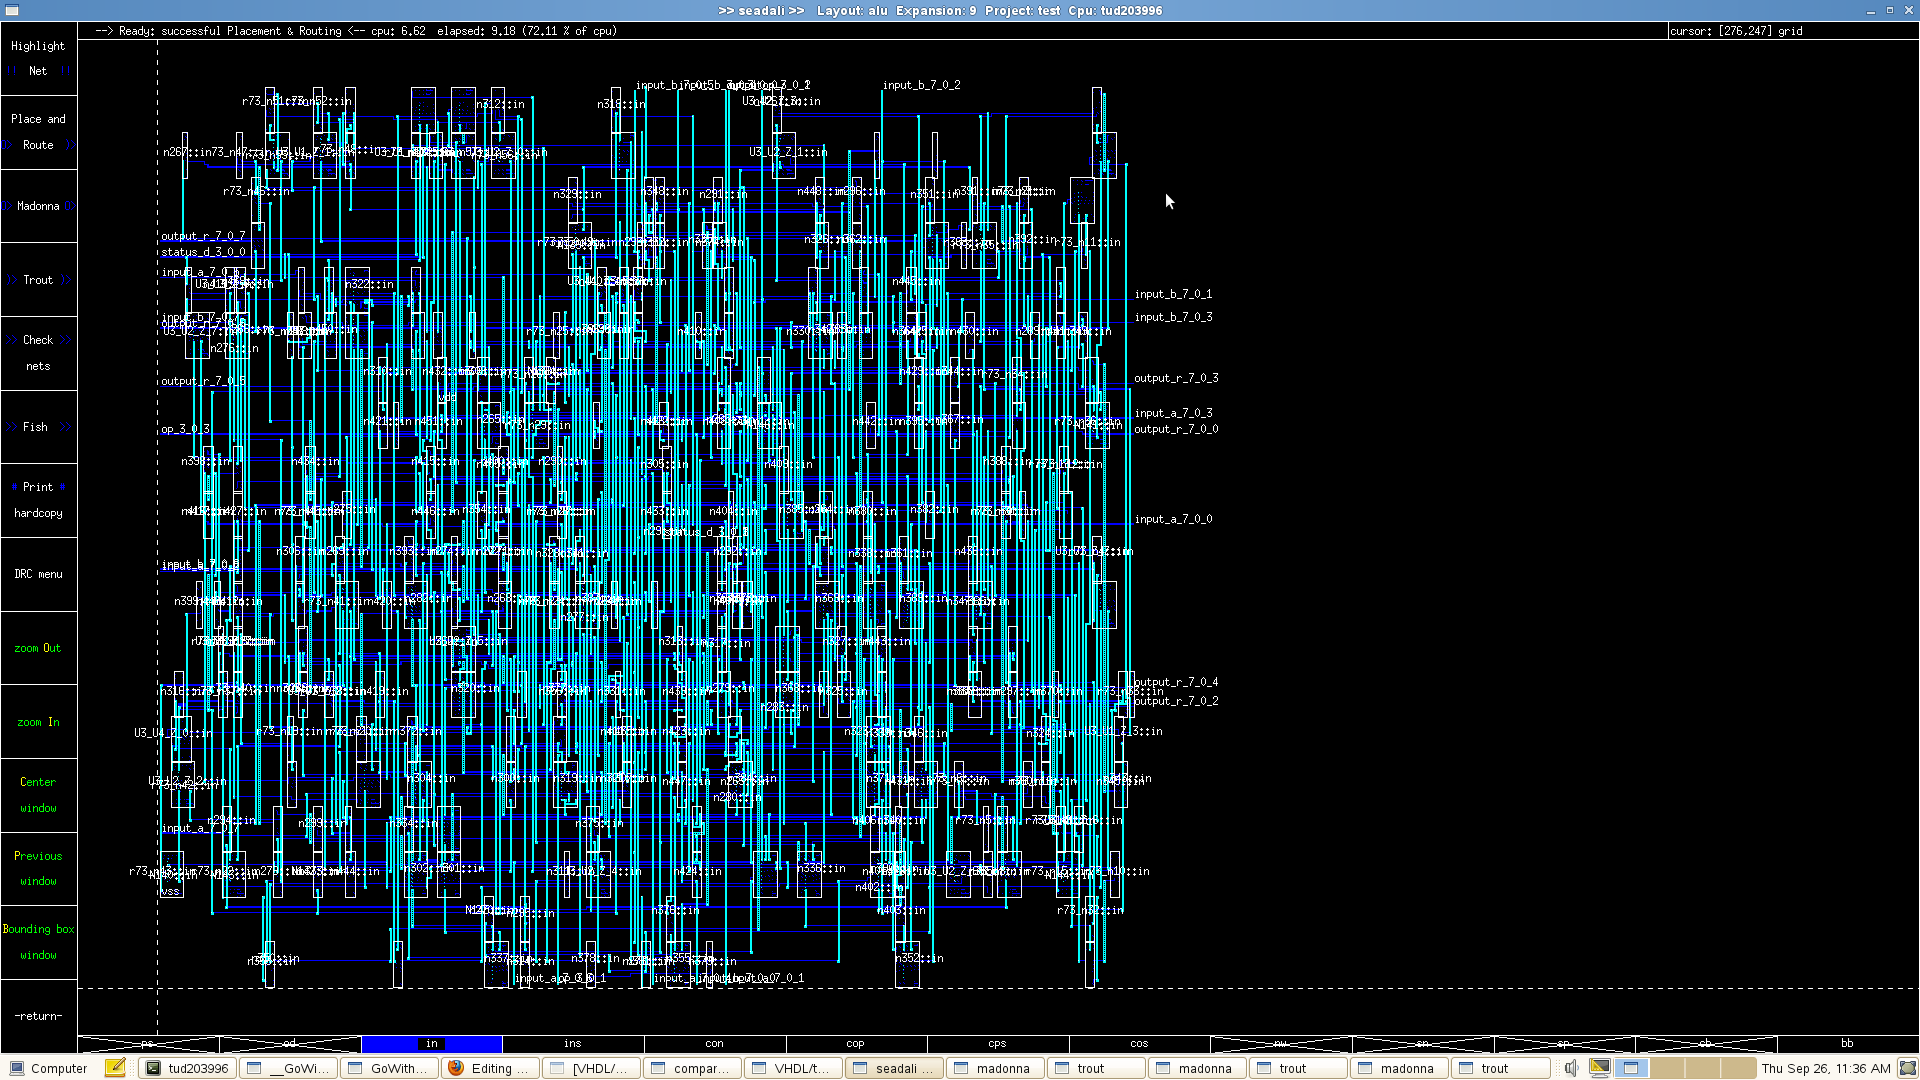
\includegraphics [width=\linewidth]{figures/lay-out}
\caption{De layout van de alu}
\label{a}
\end{figure}

%nog plaatjes includen
%Switch-level/Spice simulatieresultaten van de uit de layout ge-extraheerde schakeling.
Er zijn twee manieren om de schakeling te verifieren. De eerste is op switch level niveau. Hierbij wordt vanuit de layout een VHDL-beschrijving geëxtraheerd. Deze wordt dan met ModelSim gesimuleerd. Het resultaat hiervan staat in figuur \ref{b}.
\begin{figure} [h!]
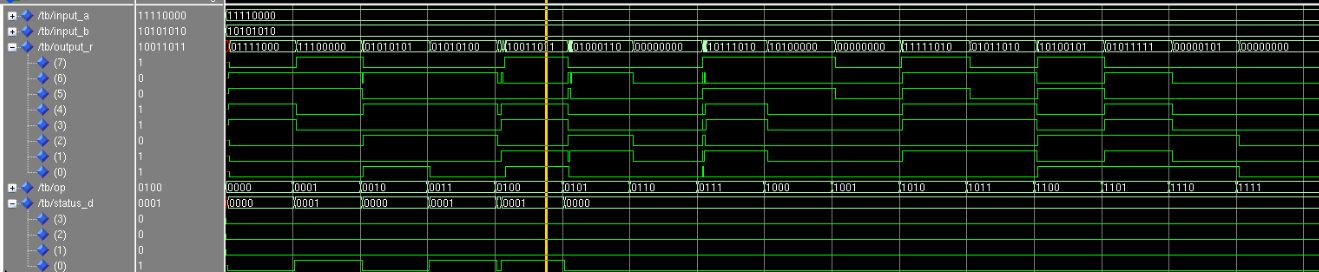
\includegraphics [width=\linewidth]{figures/sim_extractedd}
\caption{Verificatie op layout/Modelsim niveau}
\label{b}
\end{figure}
De andere manier gaat dieper. Hierbij wordt  een uit de layout geëxtraheerde transistorbeschrijving gesimuleerd. Het resultaat hiervan staat in 
\begin{figure} [h!]
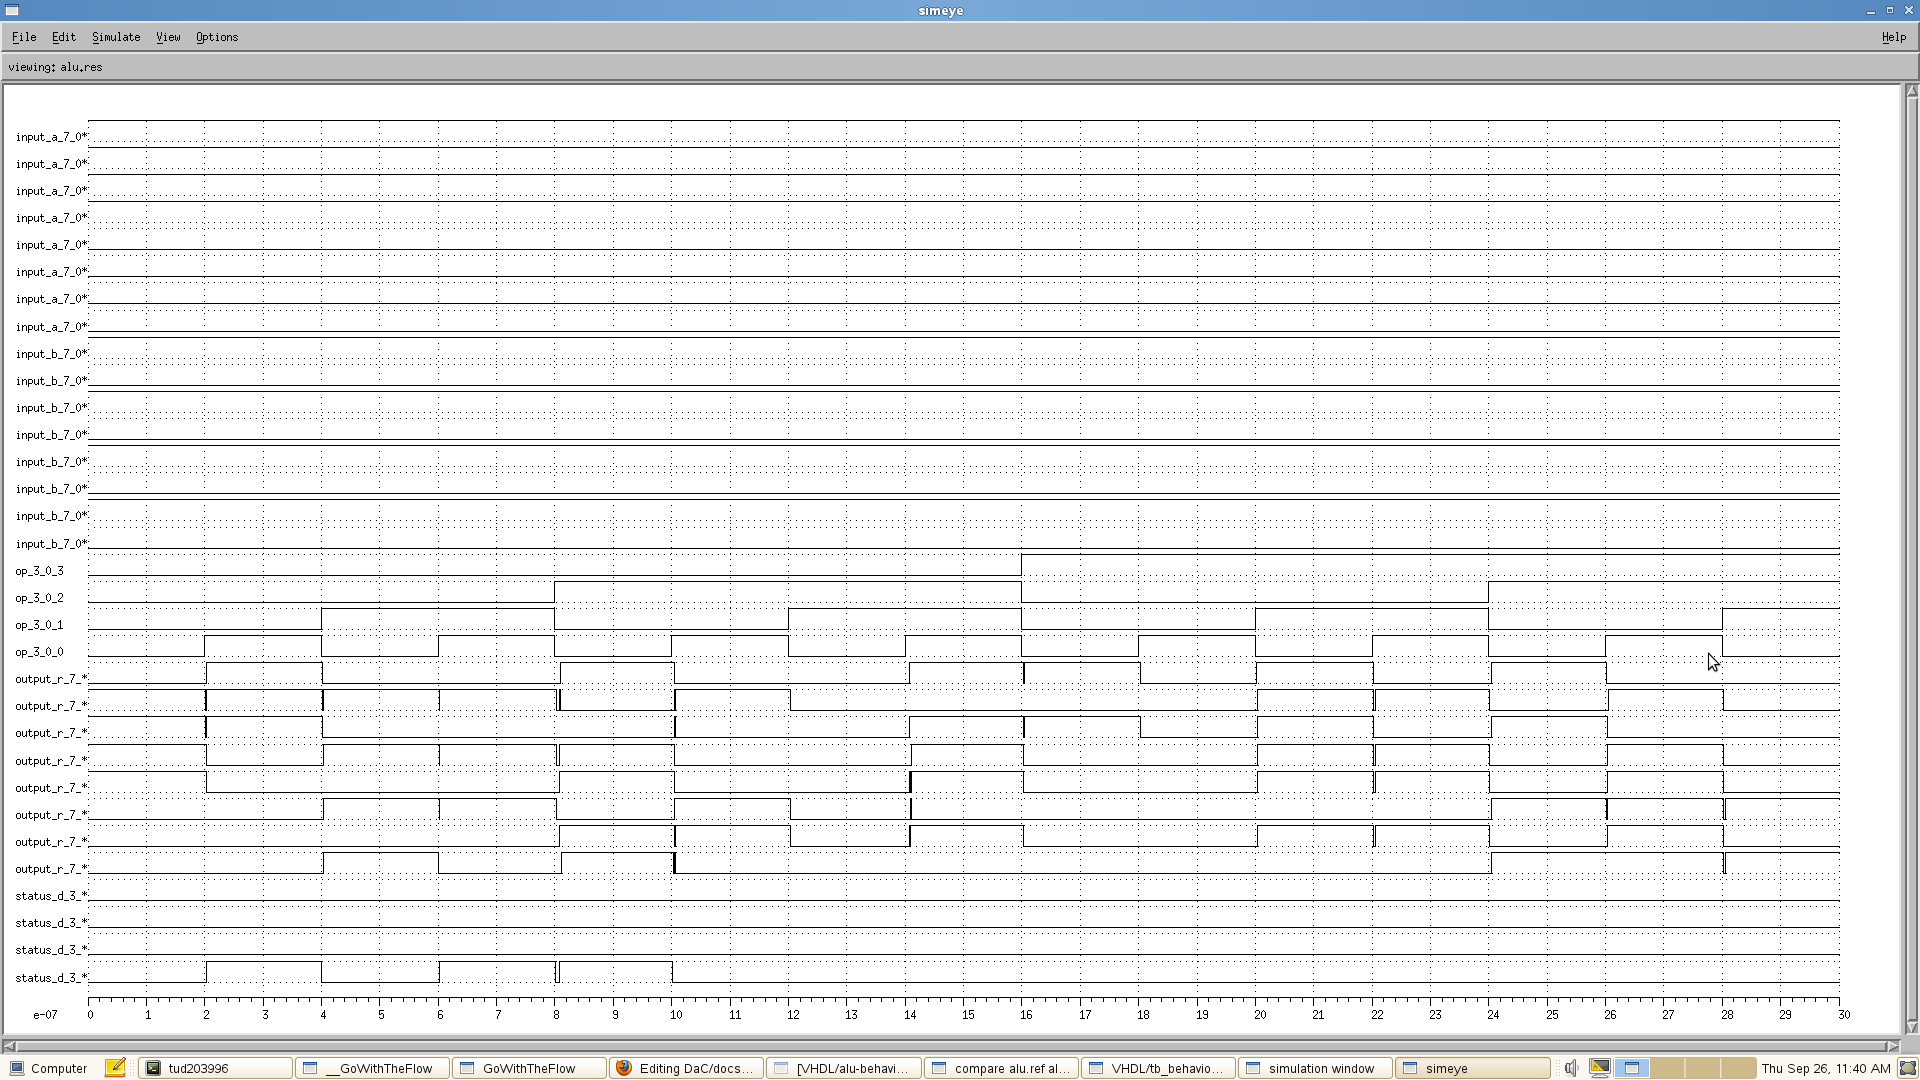
\includegraphics [width=\linewidth]{figures/switch-level}
\caption{Verificatie op transistor beschrijvingsniveau}
\label{a}
\end{figure}
Dan kunnen deze beide simulaties nog vergeleken worden door GoWithTheFlow. Het resultaat daarvan staat in figuur \ref{c}. Aan de figuur is te zien dat er geen verschillen zijn. Eerst was er 1 verschil doordat de carry in het ene geval wél en in het andere geval niet mee werd genomen. Dat is, zoals hierboven beschreven, opgelost. 
\begin{figure} [h!]
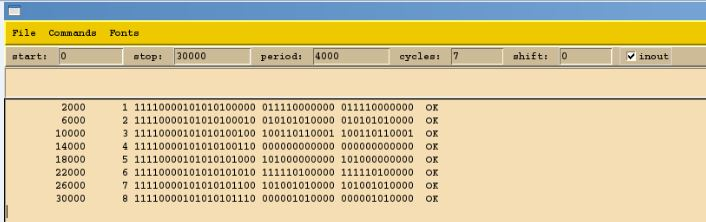
\includegraphics [width=\linewidth]{figures/comparez}
\caption{Het vergelijken van de twee simulaties}
\label{c}
\end{figure}




\end{document}










